\documentclass{report}

\input{preamble}
\input{macros}
\input{letterfonts}

\usepackage{tikz}
\usepackage{tikz-3dplot}
\usepackage{amsmath}
\usepackage{amssymb}
\usepackage{pgfplots}
\usepgfplotslibrary{polar}
\pgfplotsset{compat=newest}
\usepackage{smartdiagram}
\usepackage{xcolor}
\usepackage{forest}
\usepgfplotslibrary{colormaps}
\usepgfplotslibrary{groupplots}

%added
\tikzset{>=latex}
\usepackage{siunitx}
\usepackage[outline]{contour} % glow around text
\usetikzlibrary{angles,quotes} % for pic
\contourlength{1.3pt}
\usetikzlibrary{math}
\usepackage{ifthen}
\tikzset{>=latex} % for LaTeX arrow head
\usepackage{xcolor}
\colorlet{veccol}{green!70!black}
\colorlet{vcol}{green!70!black}
\colorlet{xcol}{blue!85!black}
\colorlet{projcol}{xcol!60}
\colorlet{unitcol}{xcol!60!black!85}
\colorlet{unitcol2}{vcol!60!black!85}
\colorlet{myblue}{blue!70!black}
\colorlet{myred}{red!70!black}
\tikzstyle{vector}=[->,very thick,xcol]
\tikzstyle{mydashed}=[dash pattern=on 2pt off 2pt]
\def\tick#1#2{\draw[thick] (#1) ++ (#2:0.1) --++ (#2-180:0.2)} %0.03*\xmax


\usesmartdiagramlibrary{additions}

\title{\Huge{Temporary Doc}\\Calc 3}
\author{\huge{Giacomo Cappelletto}}
\date{23/10/24}

\begin{document}


\maketitle
\pagebreak
\pdfbookmark[section]{\contentsname}{toc}
\tableofcontents
\pagebreak


\chapter{Vector Valued Functions $f:\mathbb{R} \rightarrow \mathbb{R}^n$}

\section{Change of Variable for Double and Triple Integrals}

\subsection*{Polar Coordinates}
\[
	\iint_D f(x, y) \, dx \, dy \rightarrow \iint_S f(r\cos\theta, r\sin\theta) \, r \, dr \, d\theta
\]

\subsection*{Cylindrical Coordinates}
\[
	\iiint_D f(x, y, z) \, dx \, dy \, dz \rightarrow \iiint_S f(r\cos\theta, r\sin\theta, z) \, r \, dr \, d\theta \, dz
\]

\subsection*{Spherical Coordinates}
\[
	\iiint_D f(x, y, z) \, dx \, dy \, dz \rightarrow \iiint_S f(\rho\sin\phi\cos\theta, \rho\sin\phi\sin\theta, \rho\cos\phi) \, \rho^2 \sin\phi \, d\rho \, d\phi \, d\theta
\]

\thm{Intuition Behind Change of Variables}{
We use a \textbf{mapping} \( T \) to transform coordinates in one space \( S \) to another \( R \). This is particularly useful when integrating over regions that are easier to describe in new coordinates (e.g., circular or spherical regions).

For example:
\[
	S = [0, 2\pi] \times [0, 2], \quad T(r, \theta) = (r\cos\theta, r\sin\theta)
\]

Here, the mapping \( T \) converts a point in \( S \) into a point in \( R \).


\subsection*{Area Differential Transformation}
Consider a small differential area element in the original space:
\[
	dA = |\det(J)| \, du \, dv
\]
where \( J \) is the \textbf{Jacobian matrix}, and \( |\det(J)| \) accounts for how the transformation scales area.
}

\dfn{Jacobian Matrix}{
	The Jacobian matrix represents the linear transformation of the mapping \( T \) at a given point:
	\[
		J = \begin{bmatrix}
			\frac{\partial x}{\partial u} & \frac{\partial x}{\partial v} \\
			\frac{\partial y}{\partial u} & \frac{\partial y}{\partial v}
		\end{bmatrix}
	\]

	For a transformation \( T(u, v) = (g(u, v), h(u, v)) \), the determinant of \( J \) is:
	\[
		\det(J) =
		\begin{vmatrix}
			\frac{\partial g}{\partial u} & \frac{\partial g}{\partial v} \\
			\frac{\partial h}{\partial u} & \frac{\partial h}{\partial v}
		\end{vmatrix}
		= \frac{\partial g}{\partial u} \cdot \frac{\partial h}{\partial v} - \frac{\partial g}{\partial v} \cdot \frac{\partial h}{\partial u}
	\]

}

\subsection*{Geometric Interpretation}
\begin{itemize}
	\item \textbf{Local Stretching/Scaling:} \( |\det(J)| \) gives the local scaling factor of the area due to the transformation.
	\item \textbf{Orientation:} The sign of \( \det(J) \) indicates whether the orientation is preserved or flipped.
\end{itemize}

\ex{Polar Coordinates}{
	For the transformation \( T(r, \theta) = (r\cos\theta, r\sin\theta) \), the Jacobian matrix is:
	\[
		J = \begin{bmatrix}
			\cos\theta & -r\sin\theta \\
			\sin\theta & r\cos\theta
		\end{bmatrix}
	\]

	The determinant is:
	\[
		\det(J) = \begin{vmatrix}
			\cos\theta & -r\sin\theta \\
			\sin\theta & r\cos\theta
		\end{vmatrix}
		= r(\cos^2\theta + \sin^2\theta) = r
	\]

	Thus, the area differential in polar coordinates becomes:
	\[
		dx \, dy = r \, dr \, d\theta
	\]

}

\dfn{General Formula for Transforming Integrals}{
	If \( T: S \rightarrow R \) is a transformation with Jacobian determinant \( |\det(J)| \), then the integral transforms as:
	\[
		\iint_R f(x, y) \, dx \, dy = \iint_S f(T(u, v)) \, |\det(J)| \, du \, dv
	\]

}

\dfn{Intuition for Higher Dimensions}{
	In three dimensions, the Jacobian matrix extends to account for the transformation of volume elements:
	\[
		J = \begin{bmatrix}
			\frac{\partial x}{\partial u} & \frac{\partial x}{\partial v} & \frac{\partial x}{\partial w} \\
			\frac{\partial y}{\partial u} & \frac{\partial y}{\partial v} & \frac{\partial y}{\partial w} \\
			\frac{\partial z}{\partial u} & \frac{\partial z}{\partial v} & \frac{\partial z}{\partial w}
		\end{bmatrix}
	\]

	The volume scaling factor is given by \( |\det(J)| \), and the integral transforms as:
	\[
		\iiint_R f(x, y, z) \, dx \, dy \, dz = \iiint_S f(T(u, v, w)) \, |\det(J)| \, du \, dv \, dw
	\]

}

\section{Non-overlapping from Mapping \( T \)}

\thm{Non-overlapping Condition}{
	For any two points \( Q \) and \( P \):
	\[
		T(Q) \neq T(P) \quad \text{(This would result in overlapping areas in the domain \( R \))}
	\]
	However, boundaries (e.g., \( y = 2x \)) can overlap as long as the bounded region is distinct.
}

\ex{Integral Transformation Example}{
	Evaluate:
	\[
		\iint_R 2x(y - 2x) \, dA
	\]
	where \( R \) is the parallelogram with vertices \((0, 0), (0, 1), (2, 4), (2, 3)\).

	Steps:
	\begin{enumerate}
		\item \textbf{Choose a Transformation:} Select a mapping \( T \) to simplify the integral.
		\item \textbf{Define the Mapping:}
		      \[
			      x = u, \quad y = 2x + v = 2u + v
		      \]
		      Substituting:
		      \[
			      (x, y) \rightarrow (u, v)
		      \]

		\item \textbf{Boundary Equations:}
		      \[
			      0 \leq x \leq 2 \quad \Rightarrow \quad 0 \leq u \leq 2
		      \]
		      \[
			      0 \leq y - 2x < 1 \quad \Rightarrow \quad 0 \leq v < 1
		      \]

		\item \textbf{Region:}
		      \[
			      S = [0, 2] \times [0, 1]
		      \]

		\item \textbf{Transform the Integrand:}
		      \[
			      f(T(x, y)) = 2u(v)
		      \]

		\item \textbf{Jacobian Calculation:}
		      \[
			      J = \begin{bmatrix}
				      x_u & x_v \\
				      y_u & y_v
			      \end{bmatrix}
			      = \begin{bmatrix}
				      1 & 0 \\
				      2 & 1
			      \end{bmatrix}, \quad \det(J) = 1 \cdot 1 - 2 \cdot 0 = 1
		      \]

		\item \textbf{Transformed Integral:}
		      \[
			      \iint_R 2x(y - 2x) \, dA = \int_0^2 \int_0^1 2uv \, du \, dv
		      \]
	\end{enumerate}
}

\section{Integral Transformation for a Parallelogram Region}

\ex{Example of Transformation}{
	Evaluate:
	\[
		\iint_R 2x(y - 2x) \, dA
	\]
	where \( R \) is the parallelogram defined by the vertices \((0, 0), (0, 1), (2, 4), (2, 3)\).

	\subsection*{Steps:}
	\begin{enumerate}
		\item \textbf{Choose a Transformation:} Select a transformation \( T \) that simplifies the integral.
		\item \textbf{Define \( x, y \) in terms of \( u, v \):}
		      \[
			      x = u, \quad y = 2x + v = 2u + v
		      \]
		      Substituting:
		      \[
			      (x, y) \rightarrow (u, v)
		      \]
		      Here, \( u \) corresponds to \( x \), and \( v = y - 2x \).

		\item \textbf{Boundary Equations:}
		      \[
			      0 \leq x \leq 2 \quad \Rightarrow \quad 0 \leq u \leq 2
		      \]
		      \[
			      0 \leq y - 2x < 1 \quad \Rightarrow \quad 0 \leq v < 1
		      \]

		\item \textbf{Region in \( u, v \):}
		      \[
			      S = [0, 2] \times [0, 1]
		      \]
		      This maps the parallelogram \( R \) into a rectangle \( S \) in the \( u, v \)-plane.

		\item \textbf{Transform the Integrand:}
		      Substituting \( x = u \) and \( y - 2x = v \):
		      \[
			      f(T(x, y)) = 2u(v)
		      \]

		\item \textbf{Jacobian Calculation:}
		      The Jacobian matrix for the transformation \( T \) is:
		      \[
			      J = \begin{bmatrix}
				      x_u & x_v \\
				      y_u & y_v
			      \end{bmatrix}
			      = \begin{bmatrix}
				      1 & 0 \\
				      2 & 1
			      \end{bmatrix}
		      \]
		      The determinant of \( J \) is:
		      \[
			      \det(J) = 1 \cdot 1 - 2 \cdot 0 = 1
		      \]

		\item \textbf{Transformed Integral:}
		      Using the transformation and the Jacobian determinant:
		      \[
			      \iint_R 2x(y - 2x) \, dA = \int_0^2 \int_0^1 2uv \, du \, dv
		      \]
		      The transformed integral simplifies the computation significantly.
	\end{enumerate}
}

\section{Integral Transformation for a Triangular Region}

\ex{Example of Transformation}{
	Evaluate:
	\[
		\iint_R (x - u)\sqrt{x - 2y} \, dA
	\]
	where \( R \) is the triangular region bounded by the lines \( y = 0 \), \( x - 2y = 0 \), and \( x = y + 1 \).

	\subsection*{Steps:}
	\begin{enumerate}
		\item \textbf{Region Definition:}
		      The region \( R \) is defined by:
		      \[
			      y = 0, \quad x - 2y = 0, \quad x = y + 1
		      \]
		      The boundaries in \( x \) and \( y \) are:
		      \[
			      0 \leq x \leq 2, \quad 0 \leq y \leq \frac{x}{2}, \quad x \leq y + 1
		      \]

		\item \textbf{Define Transformation:}
		      Let:
		      \[
			      u = x - 2y, \quad v = x - y
		      \]
		      Substituting:
		      \[
			      x = v + u, \quad y = v - u
		      \]

		\item \textbf{Boundaries in New Coordinates:}
		      Using the transformation:
		      \begin{align*}
			      u & = x - 2y \quad \Rightarrow \quad 0 \leq u \leq 1 \\
			      v & = x - y \quad \Rightarrow \quad u \leq v \leq 1
		      \end{align*}

		      The transformed region \( S \) is bounded by \( u = 0 \), \( v = 1 \), and \( v - u = 1 \).

		\item \textbf{Jacobian Calculation:}
		      The Jacobian matrix for the transformation \( T(u, v) \) is:
		      \[
			      J = \begin{bmatrix}
				      \frac{\partial x}{\partial u} & \frac{\partial x}{\partial v} \\
				      \frac{\partial y}{\partial u} & \frac{\partial y}{\partial v}
			      \end{bmatrix}
			      = \begin{bmatrix}
				      1  & 1 \\
				      -2 & 1
			      \end{bmatrix}
		      \]
		      The determinant of \( J \) is:
		      \[
			      \det(J) = (1)(1) - (1)(-2) = 1 + 2 = 3
		      \]

		\item \textbf{Transform the Integral:}
		      Using the transformation and Jacobian determinant:
		      \[
			      \iint_R (x - u)\sqrt{x - 2y} \, dA = \int_0^1 \int_0^v \sqrt{u} \cdot 3 \, du \, dv
		      \]
		      Simplify:
		      \[
			      \int_0^1 \int_0^v \sqrt{u} \, du \, dv = \int_0^1 \left[ \frac{2}{3} u^{3/2} \right]_0^v dv
			      = \int_0^1 \frac{2}{3} v^{3/2} dv
		      \]
		      \[
			      = \left[ \frac{2}{3} \cdot \frac{2}{5} v^{5/2} \right]_0^1 = \frac{4}{15}.
		      \]
		      The result is:
		      \[
			      \iint_R (x - u)\sqrt{x - 2y} \, dA = \frac{4}{15}.
		      \]
	\end{enumerate}
}


\chapter{Vector Fields $f:\mathbb{R}^n \rightarrow \mathbb{R}^n$}


\section{Vector Fields}

A \textbf{vector field} is a function $\vec{F}$ that takes points in $\mathbb{R}^2$ or $\mathbb{R}^3$ and outputs a vector in $\mathbb{R}^2$ or $\mathbb{R}^3$:
\[
	\vec{F} : \mathbb{R}^n \to \mathbb{R}^n, \quad \vec{F}(x, y, z) = \langle q(x, y, z), w(x, y, z), t(x, y, z) \rangle.
\]

\subsection{Properties}
\begin{itemize}
	\item Continuous if $q, w, t$ are continuous.
	\item Differentiable if $q, w, t$ are differentiable.
	\item Domain is the intersection of domains of $q, w, t$.
\end{itemize}

\subsection{Applications}
\begin{itemize}
	\item Water and wind currents.
	\item Gravitational, electric, and magnetic fields.
	\item Human circulation, heat propagation.
	\item Modeling through partial differential equations.
\end{itemize}

\subsection{Drawing a Vector Field}
At each point in the domain of $\vec{F}$, draw a vector whose:
\begin{itemize}
	\item Direction is parallel to $\vec{F}(x, y)$.
	\item Length is proportional to the magnitude of $\vec{F}(x, y)$.
\end{itemize}

\ex{$\vec{F}(x, y) = \frac{ \langle x, y \rangle }{\left\lvert \langle x, y \rangle \right\rvert ^3 } $}{
	\begin{center}
		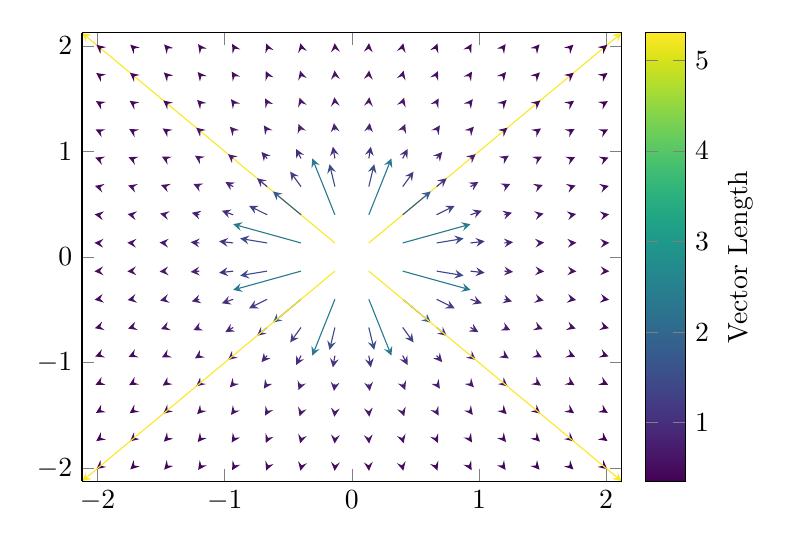
\begin{tikzpicture}
			\begin{axis}[%
					view     = {0}{90}, % for a view 'from above'
					domain   = -2:2,
					y domain = -2:2,
					xtick    = {-2,...,2},
					ytick    = {-2,...,2},
					colormap/viridis,
					colorbar,
					colorbar style = {
							ylabel = {Vector Length}
						}
				]
				\addplot3[
					point meta = {(x^2 + y^2)^(-1/2)}, % length of the vector
					quiver = {
							u = {x/(x^2+y^2)^(3/2)},
							v = {y/(x^2+y^2)^(3/2)},
							scale arrows = 0.1,
						},
					quiver/colored = {mapped color},
					-stealth,
					samples = 16
				] (x, y, 0);
			\end{axis}
		\end{tikzpicture}
	\end{center}
}

\ex{ $\vec{F}(x, y) = \langle -y, x \rangle$ }{
	\begin{center}
		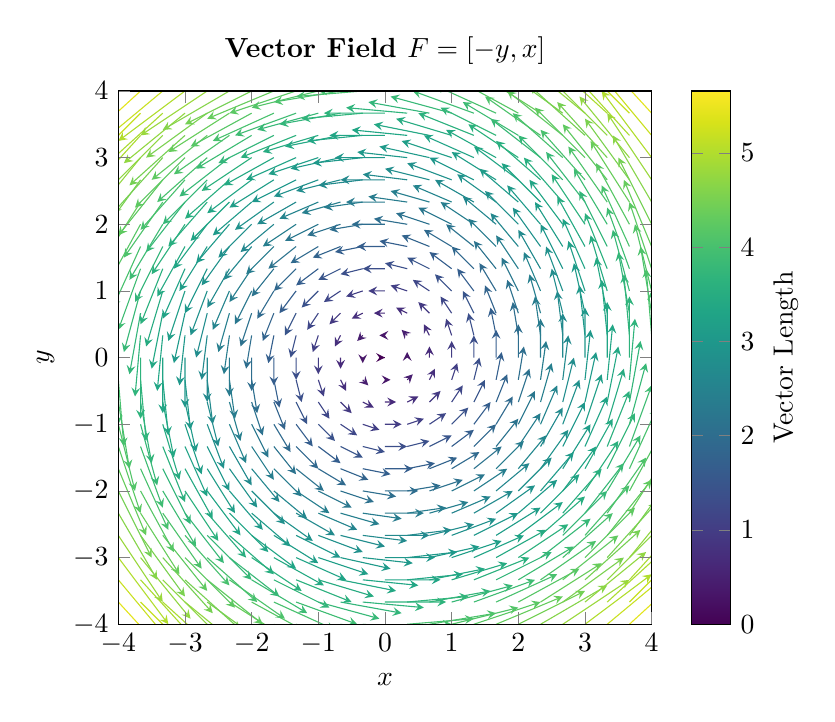
\begin{tikzpicture}
			\begin{axis}[
				xmin = -4, xmax = 4,
				ymin = -4, ymax = 4,
				zmin = 0, zmax = 1,
				axis equal image,
				xtick distance = 1,
				ytick distance = 1,
				view = {0}{90},
				scale = 1.25,
				title = {\bf Vector Field $F = [-y,x]$},
				height=7cm,
				xlabel = {$x$},
				ylabel = {$y$},
				colormap/viridis,
				colorbar,
				colorbar style = {
						ylabel = {Vector Length}
					}
				]
				\addplot3[
					point meta = {sqrt(x^2+y^2)},
					quiver = {
							u = {-y},
							v = {x},
							scale arrows = 0.25,
						},
					quiver/colored = {mapped color},
					-stealth,
					domain = -4:4,
					domain y = -4:4,
				] {0};
			\end{axis}
		\end{tikzpicture}
	\end{center}
}

\section{Gradient Vector Fields}

A \textbf{gradient vector field} $\nabla \varphi(x, y)$ is a vector field:
\[
	\vec{F}(x, y) = \nabla \varphi \quad \text{where } \varphi \text{ is a potential function.}
\]

If $\varphi$ exists, $\vec{F}$ is called a \textbf{conservative field}.

\ex{ $\varphi = -\frac{x^2 + y^2}{2}$ }{
	\[
		\vec{F}(x, y) = \nabla \varphi = \langle -x, -y \rangle
	\]
	\begin{center}
		\begin{center}
			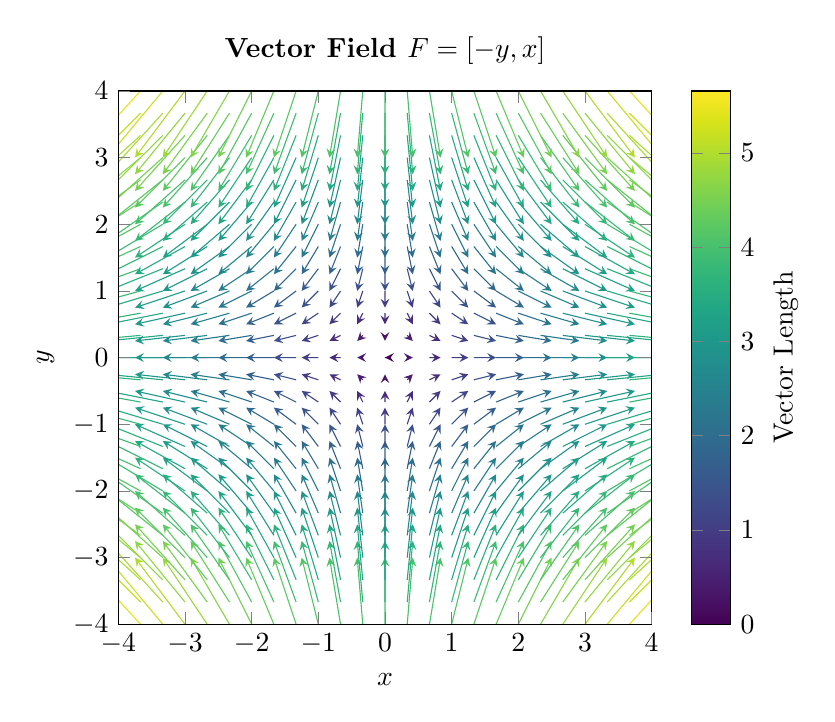
\begin{tikzpicture}
				\begin{axis}[
					xmin = -4, xmax = 4,
					ymin = -4, ymax = 4,
					zmin = 0, zmax = 1,
					axis equal image,
					xtick distance = 1,
					ytick distance = 1,
					view = {0}{90},
					scale = 1.25,
					title = {\bf Vector Field $F = [-y,x]$},
					height=7cm,
					xlabel = {$x$},
					ylabel = {$y$},
					colormap/viridis,
					colorbar,
					colorbar style = {
							ylabel = {Vector Length}
						}
					]
					\addplot3[
						point meta = {sqrt(x^2+y^2)},
						quiver = {
								u = {x},
								v = {-y},
								scale arrows = 0.25,
							},
						quiver/colored = {mapped color},
						-stealth,
						domain = -4:4,
						domain y = -4:4,
					] {0};
				\end{axis}
			\end{tikzpicture}
		\end{center}
	\end{center}
}


\section{Line Integrals}

\subsection*{Scalar Case}
For a scalar function \( f(x, y) \), the line integral over a curve \( C \) is defined as:
\[
	A = \int_C f(x, y) \, ds
\]
where \( ds = |\mathbf{r}'(t)| dt \), with \( \mathbf{r}(t) \) being the parameterization of \( C \).

If \( \mathbf{r}(t) = (x(t), y(t)) \), then:
\[
	ds = \sqrt{\left( \frac{dx}{dt} \right)^2 + \left( \frac{dy}{dt} \right)^2} \, dt
\]

This allows us to rewrite the line integral as:
\[
	\int_C f(x, y) \, ds = \int_a^b f(\mathbf{r}(t)) |\mathbf{r}'(t)| \, dt
\]

\ex{Example: Average Temperature on a Plate}{
	Suppose we have a plate located in \( R = \{(x, y) : x^2 + y^2 \leq 4 \}\), where the temperature at any point \( (x, y) \) is \( T(x, y) = 100 (x^2 + y^2) \). Find the average temperature over the boundary of \( R \).

	\begin{enumerate}
		\item \textbf{Parameterize the Boundary:}
		      The boundary \( C \) of \( R \) is a circle of radius \( 2 \), centered at the origin. Parameterize \( C \) as:
		      \[
			      \mathbf{r}(t) = (2\cos t, 2\sin t), \quad 0 \leq t \leq 2\pi
		      \]
		      Then:
		      \[
			      |\mathbf{r}'(t)| = \sqrt{(-2\sin t)^2 + (2\cos t)^2} = 2
		      \]

		\item \textbf{Average Temperature:}
		      The average temperature is given by:
		      \[
			      \text{Average Temperature} = \frac{\int_C T(x, y) \, ds}{\int_C ds}
		      \]
		      Compute the numerator:
		      \[
			      \int_C T(x, y) \, ds = \int_0^{2\pi} 100 \cdot 4 \cdot 2 \, dt = 800\pi
		      \]
		      Compute the denominator (arc length of \( C \)):
		      \[
			      \int_C ds = \int_0^{2\pi} 2 \, dt = 4\pi
		      \]
		      Thus:
		      \[
			      \text{Average Temperature} = \frac{800\pi}{4\pi} = 200
		      \]
	\end{enumerate}
}

\subsection*{Oriented Curves}
An oriented curve \( C \) includes a direction along the curve. For example, when calculating work done by a force \( \mathbf{F} \) along a curve, the direction matters.

\ex{Example: Work}{
	Work done by a force \( \mathbf{F}(x) \) is given by:
	\[
		W = \int_a^b F(x) \, dx
	\]
	For a spring with force \( F(x) = -kx \), the work done to stretch the spring from \( x = a \) to \( x = b \) is:
	\[
		W = \int_a^b -kx \, dx = -\frac{k}{2} \left[ b^2 - a^2 \right]
	\]
}

\section{Vector Line Integrals}

\ex{Example: Earth's Gravitational Field}{
	The Earth's gravitational field exerts a force \( \mathbf{F}(\mathbf{r}) \) on an object, pulling it toward the origin. Suppose an object travels along a path \( C \). The work done by \( \mathbf{F} \) is:
	\[
		W = \int_C \mathbf{F} \cdot d\mathbf{r}
	\]
	If \( \mathbf{F}(\mathbf{r}) = \frac{-Gm}{|\mathbf{r}|^3} \mathbf{r} \), parameterize \( C \) as \( \mathbf{r}(t) \), and compute:
	\[
		\mathbf{F}(\mathbf{r}) = -\frac{Gm}{|\mathbf{r}|^3} \mathbf{r}, \quad d\mathbf{r} = \mathbf{r}'(t) \, dt
	\]
	Then:
	\[
		W = \int_a^b \mathbf{F}(\mathbf{r}(t)) \cdot \mathbf{r}'(t) \, dt
	\]

	If \( C \) is along the z-axis from \( (0, 0, 1) \) to \( (0, 0, 4) \), parameterize:
	\[
		\mathbf{r}(t) = (0, 0, t), \quad 1 \leq t \leq 4
	\]
	Then:
	\[
		W = \int_1^4 -\frac{Gm}{t^2} \cdot 1 \, dt = -Gm \int_1^4 \frac{1}{t^2} \, dt
	\]
	\[
		W = -Gm \left[ -\frac{1}{t} \right]_1^4 = -Gm \left( -\frac{1}{4} + 1 \right) = Gm \left( \frac{3}{4} \right)
	\]
}

\section{Fundamental Theorem of Line Integrals}

\thm{Fundamental Theorem of Line Integrals}{
	If \( \mathbf{F} \) is a vector field that can be expressed as \( \mathbf{F} = \nabla \phi \), then given an oriented curve \( C \) from \( P \) to \( Q \):
	\[
		\int_C \mathbf{F} \cdot d\mathbf{r} = \phi(Q) - \phi(P)
	\]
}

\ex{Example}{
	Let \( \phi(x, y, z) = \frac{-G}{\sqrt{x^2 + y^2 + z^2}} \), and \( \mathbf{F} = \nabla \phi \). Compute:
	\[
		\int_C \mathbf{F} \cdot d\mathbf{r}
	\]
	from \( (a, a, a) \) to \( (1, 1, 1) \):
	\[
		\phi(x, y, z) = \frac{-G}{\sqrt{x^2 + y^2 + z^2}}, \quad \Delta \phi = \phi(1, 1, 1) - \phi(a, a, a)
	\]
	\[
		\phi(a, a, a) = \frac{-G}{\sqrt{3a^2}} = \frac{-G}{a\sqrt{3}}, \quad \phi(1, 1, 1) = \frac{-G}{\sqrt{3}}
	\]
	Thus:
	\[
		\int_C \mathbf{F} \cdot d\mathbf{r} = \phi(1, 1, 1) - \phi(a, a, a) = \frac{-G}{\sqrt{3}} - \left( \frac{-G}{a\sqrt{3}} \right)
	\]
	\[
		= \frac{G}{\sqrt{3}} \left( 1 - \frac{1}{a} \right)
	\]
}

\section{Vector Line Integrals and Gradient Fields}

\subsection{Vector Line Integral for a Curve \( C \)}
Given a vector field \( \mathbf{F}(x, y) = (P(x, y), Q(x, y)) \) and an oriented curve \( C \), the vector line integral is defined as:
\[
	\int_C \mathbf{F} \cdot d\mathbf{r} = \int_C P \, dx + Q \, dy
\]
where:
\[
	d\mathbf{r} = (dx, dy), \quad \mathbf{F} \cdot d\mathbf{r} = P \, dx + Q \, dy.
\]

If \( C \) is parameterized as \( \mathbf{r}(t) = (x(t), y(t)) \), where \( t \in [a, b] \), then:
\[
	\int_C \mathbf{F} \cdot d\mathbf{r} = \int_a^b \mathbf{F}(\mathbf{r}(t)) \cdot \mathbf{r}'(t) \, dt = \int_a^b \left[ P(x(t), y(t)) \frac{dx}{dt} + Q(x(t), y(t)) \frac{dy}{dt} \right] dt
\]

\ex{Example: Compute a Vector Line Integral}{
	Let \( \mathbf{F}(x, y) = (x, x^2 + y) \) and let \( C \) be the curve defined by \( \mathbf{r}(t) = (t, t^2) \), where \( t \in [1, 3] \).

	\textbf{Steps:}
	\begin{enumerate}
		\item \textbf{Parameterize \( C \):}
		      From the parameterization, we have:
		      \[
			      x(t) = t, \quad y(t) = t^2, \quad \mathbf{r}'(t) = \left(\frac{dx}{dt}, \frac{dy}{dt}\right) = (1, 2t)
		      \]

		\item \textbf{Evaluate \( \mathbf{F}(\mathbf{r}(t)) \cdot \mathbf{r}'(t) \):}
		      Substitute \( x(t) \) and \( y(t) \) into \( \mathbf{F}(x, y) \):
		      \[
			      \mathbf{F}(\mathbf{r}(t)) = (t, t^2 + t^2) = (t, 2t^2)
		      \]
		      Then:
		      \[
			      \mathbf{F}(\mathbf{r}(t)) \cdot \mathbf{r}'(t) = t \cdot 1 + (2t^2) \cdot (2t) = t + 4t^3
		      \]

		\item \textbf{Compute the Integral:}
		      \[
			      \int_C \mathbf{F} \cdot d\mathbf{r} = \int_1^3 (t + 4t^3) \, dt
		      \]
		      Split the integral:
		      \[
			      \int_1^3 (t + 4t^3) \, dt = \int_1^3 t \, dt + \int_1^3 4t^3 \, dt
		      \]
		      Compute each term:
		      \[
			      \int_1^3 t \, dt = \left[\frac{t^2}{2}\right]_1^3 = \frac{9}{2} - \frac{1}{2} = 4
		      \]
		      \[
			      \int_1^3 4t^3 \, dt = 4 \left[\frac{t^4}{4}\right]_1^3 = \left[81 - 1\right] = 80
		      \]
		      Thus:
		      \[
			      \int_C \mathbf{F} \cdot d\mathbf{r} = 4 + 80 = 84
		      \]
	\end{enumerate}
}

\subsection{Gradient Fields and Fundamental Theorem of Line Integrals}
If \( \mathbf{F} \) is a gradient field, meaning \( \mathbf{F} = \nabla \phi \), then the line integral over a curve \( C \) depends only on the endpoints of \( C \). Specifically:
\[
	\int_C \mathbf{F} \cdot d\mathbf{r} = \phi(B) - \phi(A)
\]
where \( A \) and \( B \) are the start and end points of \( C \).

\textbf{Intuition:}
\begin{itemize}
	\item The integral \( \int_C \mathbf{F} \cdot d\mathbf{r} \) represents the difference in potential between the endpoints of \( C \).
	\item The path taken does not matter; only the values of \( \phi \) at \( A \) and \( B \) are relevant.
\end{itemize}

\ex{Example: Gradient Field Integral}{
	Let \( \mathbf{F} = \nabla \phi \), where \( \phi(x, y) = x^2 + xy \). Compute:
	\[
		\int_C \mathbf{F} \cdot d\mathbf{r}
	\]
	where \( C \) is any curve starting at \( A = (1, 2) \) and ending at \( B = (3, 4) \).

	\textbf{Solution:}
	\begin{enumerate}
		\item Compute \( \phi(A) \) and \( \phi(B) \):
		      \[
			      \phi(A) = (1)^2 + (1)(2) = 1 + 2 = 3
		      \]
		      \[
			      \phi(B) = (3)^2 + (3)(4) = 9 + 12 = 21
		      \]

		\item Apply the Fundamental Theorem:
		      \[
			      \int_C \mathbf{F} \cdot d\mathbf{r} = \phi(B) - \phi(A) = 21 - 3 = 18
		      \]
	\end{enumerate}
}

\section{Gradient Vector Fields and Closed Curves}

\subsection{Definition of a Closed Curve}
A curve \( C \) is said to be \textbf{closed} if its start and end points are the same, i.e., \( A = B \).

For a closed curve \( C \), the following property holds:
\[
\int_C \mathbf{F} \cdot d\mathbf{r} = 0 \quad \text{if } \mathbf{F} \text{ is a gradient vector field}.
\]

If \( \mathbf{F} = \nabla \phi \), then:
\[
\int_C \mathbf{F} \cdot d\mathbf{r} = \phi(A) - \phi(A) = 0.
\]

This implies that \textbf{the line integral of a gradient field over a closed curve is always zero}.

\subsection{How to Identify a Gradient Vector Field}
To determine whether a vector field \( \mathbf{F} = (P(x, y), Q(x, y)) \) is a gradient field:
\begin{itemize}
    \item \( \mathbf{F} \) must be defined on a region \( R \) that is \textbf{connected} and \textbf{simply connected} (no holes in \( R \)).
    \item \( P(x, y) \) and \( Q(x, y) \) must satisfy the condition:
    \[
    \frac{\partial P}{\partial y} = \frac{\partial Q}{\partial x}.
    \]
\end{itemize}

\textbf{Theorem:} If \( \mathbf{F} \) satisfies the above conditions, then \( \mathbf{F} \) is a gradient vector field, and there exists a scalar function \( \phi(x, y) \) such that \( \mathbf{F} = \nabla \phi \).

\subsection{Finding the Potential Function \( \phi(x, y) \)}
To find \( \phi(x, y) \), follow these steps:
\begin{enumerate}
    \item Check if \( \mathbf{F} \) satisfies \( \frac{\partial P}{\partial y} = \frac{\partial Q}{\partial x} \).
    \item Assume \( \phi(x, y) \) exists and satisfies:
    \[
    \frac{\partial \phi}{\partial x} = P(x, y), \quad \frac{\partial \phi}{\partial y} = Q(x, y).
    \]
    \item Integrate \( P(x, y) \) with respect to \( x \) to find a partial expression for \( \phi(x, y) \):
    \[
    \phi(x, y) = \int P(x, y) \, dx + h(y),
    \]
    where \( h(y) \) is an arbitrary function of \( y \).
    \item Differentiate the result with respect to \( y \), and equate it to \( Q(x, y) \) to find \( h'(y) \):
    \[
    \frac{\partial \phi}{\partial y} = \frac{\partial}{\partial y} \left[ \int P(x, y) \, dx + h(y) \right] = Q(x, y).
    \]
    Solve for \( h(y) \).
    \item Substitute \( h(y) \) back into \( \phi(x, y) \) to obtain the full potential function.
\end{enumerate}

\ex{Example: Finding the Potential Function}{
Given \( \mathbf{F} = (2xy, x^2 + 2y) \), determine if \( \mathbf{F} \) is a gradient field and, if so, find \( \phi(x, y) \).

\textbf{Step 1: Check the Condition.}
\[
\frac{\partial P}{\partial y} = \frac{\partial}{\partial y} (2xy) = 2x, \quad \frac{\partial Q}{\partial x} = \frac{\partial}{\partial x} (x^2 + 2y) = 2x.
\]
Since \( \frac{\partial P}{\partial y} = \frac{\partial Q}{\partial x} \), \( \mathbf{F} \) is a gradient field.

\textbf{Step 2: Integrate \( P(x, y) \) with Respect to \( x \).}
\[
\phi(x, y) = \int P(x, y) \, dx = \int 2xy \, dx = x^2y + h(y),
\]
where \( h(y) \) is an arbitrary function of \( y \).

\textbf{Step 3: Differentiate with Respect to \( y \).}
\[
\frac{\partial \phi}{\partial y} = \frac{\partial}{\partial y} \left( x^2y + h(y) \right) = x^2 + h'(y).
\]

\textbf{Step 4: Equate to \( Q(x, y) \).}
\[
x^2 + h'(y) = x^2 + 2y \quad \Rightarrow \quad h'(y) = 2y.
\]

\textbf{Step 5: Solve for \( h(y) \).}
\[
h(y) = \int 2y \, dy = y^2 + C.
\]

\textbf{Step 6: Write the Final Potential Function.}
\[
\phi(x, y) = x^2y + y^2 + C.
\]
}

\section{Non-Gradient Vector Fields and Green's Theorem}

\subsection{Non-Gradient Vector Fields}
For a vector field \( \mathbf{F} = (P(x, y), Q(x, y)) \), if:
\[
\frac{\partial P}{\partial y} \neq \frac{\partial Q}{\partial x},
\]
then \( \mathbf{F} \) is \textbf{not a gradient vector field}.

To measure the \textbf{rotation} of \( \mathbf{F} \), we compute the \textbf{curl} of \( \mathbf{F} \), defined as:
\[
\text{curl}(\mathbf{F}) = \frac{\partial Q}{\partial x} - \frac{\partial P}{\partial y}.
\]
The curl describes the tendency of \( \mathbf{F} \) to "rotate" around a point.

\ex{Example: Interpreting the Curl}{
Suppose \( \mathbf{F}(x, y) \) represents the velocity of a fluid. If:
\[
\frac{\partial Q}{\partial x} > \frac{\partial P}{\partial y},
\]
then \( \text{curl}(\mathbf{F}) > 0 \), indicating counterclockwise rotation of the fluid flow. Conversely, if:
\[
\frac{\partial Q}{\partial x} < \frac{\partial P}{\partial y},
\]
then \( \text{curl}(\mathbf{F}) < 0 \), indicating clockwise rotation of the fluid flow.

Consider a case where \( Q_x = 1 \) and \( P_y = 0 \). This means \( \text{curl}(\mathbf{F}) = 1 \), indicating counterclockwise rotation.
}

\subsection{Green's Theorem}
Green's Theorem provides a relationship between a line integral over a closed curve \( C \) and a double integral over the region \( R \) enclosed by \( C \). 

\textbf{Theorem:}
Let \( C \) be a positively oriented, simple, closed curve enclosing a region \( R \). If \( \mathbf{F} = (P, Q) \) is a continuously differentiable vector field, then:
\[
\int_C \mathbf{F} \cdot d\mathbf{r} = \int_C P \, dx + Q \, dy = \iint_R \left( \frac{\partial Q}{\partial x} - \frac{\partial P}{\partial y} \right) \, dA.
\]

\textbf{Intuition:}
Green's Theorem states that the circulation of \( \mathbf{F} \) along the boundary \( C \) equals the sum of the curl of \( \mathbf{F} \) over the area \( R \). It connects the local rotation of \( \mathbf{F} \) (through curl) to its global behavior along the curve \( C \).

\ex{Example: Application of Green's Theorem}{
Let \( \mathbf{F} = (-3y, 3x) \), and let \( R \) be the triangle with vertices \( (0, 0), (1, 0), (0, 2) \), oriented counterclockwise. Compute \( \int_C \mathbf{F} \cdot d\mathbf{r} \) using Green's Theorem.

\textbf{Solution:}
\begin{enumerate}
    \item Compute the Curl of \( \mathbf{F} \):
    \[
    \text{curl}(\mathbf{F}) = \frac{\partial Q}{\partial x} - \frac{\partial P}{\partial y} = 3 - (-3) = 6.
    \]

    \item Set up the Double Integral over \( R \):
    The region \( R \) is the triangle with vertices \( (0, 0), (1, 0), (0, 2) \). Its boundaries can be described by:
    \[
    0 \leq x \leq 1, \quad 0 \leq y \leq 2 - 2x.
    \]
    Using Green's Theorem:
    \[
    \int_C \mathbf{F} \cdot d\mathbf{r} = \iint_R \text{curl}(\mathbf{F}) \, dA = \iint_R 6 \, dA.
    \]

    \item Compute the Double Integral:
    \[
    \iint_R 6 \, dA = \int_0^1 \int_0^{2 - 2x} 6 \, dy \, dx.
    \]
    First, integrate with respect to \( y \):
    \[
    \int_0^{2 - 2x} 6 \, dy = 6y \Big|_0^{2 - 2x} = 6(2 - 2x).
    \]
    Now integrate with respect to \( x \):
    \[
    \int_0^1 6(2 - 2x) \, dx = \int_0^1 (12 - 12x) \, dx = \left[ 12x - 6x^2 \right]_0^1.
    \]
    Evaluate:
    \[
    \left[ 12(1) - 6(1)^2 \right] - \left[ 12(0) - 6(0)^2 \right] = 12 - 6 = 6.
    \]

    \item Final Answer:
    \[
    \int_C \mathbf{F} \cdot d\mathbf{r} = 6.
    \]
\end{enumerate}
}

\section{Line Integrals and Area}

\subsection*{Area Using Line Integrals}
For a vector field \( \mathbf{F} = (-y, x) \), the curl is given by:
\[
\text{curl}(\mathbf{F}) = \frac{\partial Q}{\partial x} - \frac{\partial P}{\partial y} = 1.
\]
If \( C \) is a closed curve oriented counterclockwise, enclosing a region \( R \), the area of \( R \) can be computed using the following line integrals:
\[
\text{Area}(R) = \iint_R 1 \, dA = \int_C \mathbf{F} \cdot d\mathbf{r}.
\]
The parametrized curve \( C \) is expressed as \( \mathbf{r}(t) = (x(t), y(t)) \), with:
\[
\mathbf{F} \cdot d\mathbf{r} = P \, dx + Q \, dy.
\]

\subsection*{Alternative Formulas for Area}
Using line integrals:
\[
\text{Area}(R) = \int_C x \, dy = -\int_C y \, dx = \frac{1}{2} \int_C (x \, dy - y \, dx).
\]
These expressions are equivalent and depend on how \( C \) is parameterized.

\ex{Example: Area of an Ellipse}{
Consider an ellipse parameterized by:
\[
\mathbf{r}(t) = (a\cos t, b\sin t), \quad t \in [0, 2\pi].
\]
Here, \( a \) and \( b \) are the semi-major and semi-minor axes, respectively.

\textbf{Steps:}
\begin{enumerate}
    \item Compute \( x \, dy \):
    \[
    x = a\cos t, \quad dy = \frac{d}{dt}(b\sin t) \, dt = b\cos t \, dt.
    \]
    Thus:
    \[
    x \, dy = a\cos t \cdot b\cos t \, dt = ab\cos^2 t \, dt.
    \]

    \item Compute \( y \, dx \):
    \[
    y = b\sin t, \quad dx = \frac{d}{dt}(a\cos t) \, dt = -a\sin t \, dt.
    \]
    Thus:
    \[
    y \, dx = b\sin t \cdot (-a\sin t) \, dt = -ab\sin^2 t \, dt.
    \]

    \item Compute \( x \, dy - y \, dx \):
    \[
    x \, dy - y \, dx = ab\cos^2 t \, dt - (-ab\sin^2 t \, dt) = ab(\cos^2 t + \sin^2 t) \, dt = ab \, dt.
    \]

    \item Compute the Line Integral:
    \[
    \text{Area}(R) = \frac{1}{2} \int_0^{2\pi} ab \, dt = \frac{1}{2} ab \int_0^{2\pi} 1 \, dt = \frac{1}{2} ab \cdot 2\pi = \pi ab.
    \]
\end{enumerate}

\textbf{Conclusion:}
The area of the ellipse is:
\[
\text{Area}(R) = \pi ab,
\]
where \( a \) and \( b \) are the semi-major and semi-minor axes.
}

\subsection*{Summary}
The area of a region \( R \) enclosed by a curve \( C \) can be computed using line integrals in multiple equivalent ways:
\begin{itemize}
    \item Directly using \( \int_C \mathbf{F} \cdot d\mathbf{r} \), where \( \mathbf{F} = (-y, x) \).
    \item Using \( \int_C x \, dy \) or \( -\int_C y \, dx \).
    \item Using the symmetric formula:
    \[
    \text{Area}(R) = \frac{1}{2} \int_C (x \, dy - y \, dx).
    \]
\end{itemize}

\section{Flux of a Vector Field}

\subsection*{Definition of Flux}
Flux represents the flow of a vector field \( \mathbf{F} = (f, g) \) across an oriented curve \( C \). It measures how much of \( \mathbf{F} \) passes through \( C \) in the normal direction.

The flux of \( \mathbf{F} \) across \( C \) is defined as:
\[
\text{Flux} = \int_C \mathbf{F} \cdot \mathbf{n} \, ds,
\]
where:
\begin{itemize}
    \item \( \mathbf{n} \) is the unit normal vector to the curve \( C \).
    \item \( ds \) is the arc length differential.
\end{itemize}

For a parameterized curve \( \mathbf{r}(t) = (x(t), y(t)) \), where \( t \in [a, b] \), the unit normal vector is given by:
\[
\mathbf{n} = \frac{1}{|\mathbf{r}'(t)|} (-y'(t), x'(t)).
\]
Thus:
\[
\mathbf{F} \cdot \mathbf{n} = \frac{1}{|\mathbf{r}'(t)|} \left[f(x(t), y(t)) (-y'(t)) + g(x(t), y(t)) x'(t)\right].
\]



\subsection*{Flux in Simplified Form}
If the curve \( C \) is parameterized, the flux integral can be simplified as:
\[
\int_C \mathbf{F} \cdot \mathbf{n} \, ds = \int_a^b \left[f(x(t), y(t)) y'(t) - g(x(t), y(t)) x'(t)\right] dt.
\]
Or equivalently:
\[
\int_C \mathbf{F} \cdot \mathbf{n} \, ds = \int_C f \, dy - g \, dx.
\]



\subsection*{Green's Theorem Applied to Flux}
By applying Green's Theorem, the flux of \( \mathbf{F} = (f, g) \) across \( C \) can also be related to a double integral over the region \( R \) enclosed by \( C \):
\[
\int_C \mathbf{F} \cdot \mathbf{n} \, ds = \int_R \text{div}(\mathbf{F}) \, dA,
\]
where:
\[
\text{div}(\mathbf{F}) = \frac{\partial f}{\partial x} + \frac{\partial g}{\partial y}.
\]
This shows that the flux across the boundary \( C \) is equal to the total divergence of \( \mathbf{F} \) inside \( R \).



\ex{Example: Flux Around a Circle}{
Let \( \mathbf{F}(x, y) = (x, y) \), and let \( C \) be the circle \( x^2 + y^2 = 1 \) parameterized by:
\[
\mathbf{r}(t) = (\cos t, \sin t), \quad t \in [0, 2\pi].
\]

\textbf{Step 1: Parameterize the Flux Integral.}
The unit normal vector to \( C \) is given by:
\[
\mathbf{n} = (-\sin t, \cos t),
\]
and \( \mathbf{F}(\mathbf{r}(t)) = (\cos t, \sin t) \). Then:
\[
\mathbf{F} \cdot \mathbf{n} = \cos t (-\sin t) + \sin t (\cos t) = 0.
\]

\textbf{Step 2: Apply Green's Theorem.}
Using Green's Theorem:
\[
\int_C \mathbf{F} \cdot \mathbf{n} \, ds = \int_R \text{div}(\mathbf{F}) \, dA.
\]
The divergence of \( \mathbf{F} = (x, y) \) is:
\[
\text{div}(\mathbf{F}) = \frac{\partial x}{\partial x} + \frac{\partial y}{\partial y} = 1 + 1 = 2.
\]

The area of the circle is:
\[
\text{Area}(R) = \pi \cdot 1^2 = \pi.
\]

Thus:
\[
\int_C \mathbf{F} \cdot \mathbf{n} \, ds = \int_R 2 \, dA = 2 \cdot \pi = 2\pi.
\]

\textbf{Final Answer:}
The flux across the circle is:
\[
\text{Flux} = 2\pi.
\]
}

\end{document}